\documentclass[11pt,a4paper]{article}
\usepackage[T1]{fontenc}
\usepackage[utf8]{inputenc}
\usepackage{lmodern}
\usepackage[margin=25mm,headheight=15pt]{geometry}
\usepackage{amsmath,amssymb,amsthm,mathtools}
\usepackage{microtype,graphicx,booktabs,tabularx,array}
\usepackage[dvipsnames]{xcolor}
\usepackage{enumitem,fancyhdr}
\usepackage{hyperref}
\usepackage{bookmark}
\usepackage{url}
\hypersetup{colorlinks=true,linkcolor=MidnightBlue,citecolor=MidnightBlue,
 urlcolor=MidnightBlue,pdftitle={Li coefficients and a universal small-time Cauchy law},
 pdfauthor={ChatGPT research report prepared for Vladimir Reshetnikov}}
\urlstyle{same}
\setlength{\emergencystretch}{2em}
\setlength{\parskip}{4pt}
\setlength{\parindent}{0pt}
\setlist{itemsep=3pt,topsep=4pt}
\newtheorem{theorem}{Theorem}[section]
\newtheorem{lemma}[theorem]{Lemma}
\newtheorem{proposition}[theorem]{Proposition}
\newtheorem{corollary}[theorem]{Corollary}
\theoremstyle{definition}
\newtheorem{definition}[theorem]{Definition}
\theoremstyle{remark}
\newtheorem{remark}[theorem]{Remark}
\numberwithin{equation}{section}
\pagestyle{fancy}
\fancyhf{}
\fancyhead[L]{\small Li coefficients and a Cauchy law}
\fancyhead[R]{\small Research report / 26 November 2026}
\fancyfoot[C]{\thepage}
\renewcommand{\headrulewidth}{0.3pt}

\begin{document}
\hypersetup{pageanchor=false}
\begin{titlepage}
\vspace*{12mm}
{\color{MidnightBlue}\large MATHEMATICAL RESEARCH REPORT\par}
\vspace{8mm}
{\Huge\bfseries Li coefficients and a universal small-time Cauchy law\par}
\vspace{7mm}
{\Large An all-order density expansion, conductor universality,\par
and a bounded positive-weight sampling obstruction\par}
\vspace{12mm}
{\large Prepared for Vladimir Reshetnikov\par}
{\large 26 November 2026\par}
\vspace{10mm}
\hrule
\vspace{6mm}
\textbf{Primary inputs.} The repository
\href{https://github.com/lsernau/grh-lean}{\texttt{lsernau/grh-lean}},
revision \texttt{72fead10}, and the
Riemann hypothesis overview, followed through to primary mathematical
sources.

\textbf{Main result.} A process whose circle spectrum consists of the
real parts of Li coefficients has a Cauchy density after an exact
Lambert-$W$ rescaling. Every correction term is explicit, the expansion
holds to arbitrary order, and the error is uniform after any fixed
number of spatial derivatives.

\textbf{Second result.} A single sequence $0<a_n<4$ can give a smoothed
remainder which is zero at every fifth power and still has a Mellin pole
at $s=3/5$ with residue $1/4$. An explicit family treats all power grids
$m^p$, $p\geq4$.

\textbf{Status.} Complete mathematical proofs are provided. The new
arguments have been checked independently within this analysis and
supported by reproducible symbolic and numerical checks; they have not
been formalized in Lean. Novelty is claimed only for the precise results
identified in Section~\ref{sec:novelty}, relative to the literature
located in this investigation.
\vfill
{\small ChatGPT research report. Upstream Lean snapshots retain their
original attribution and Apache-2.0 notices.}
\end{titlepage}
\pagenumbering{arabic}
\hypersetup{pageanchor=true}

\begin{abstract}
We develop two analytic results motivated by RH, Dirichlet GRH, and the
positive-sum interfaces in the Alp\"oge--Claude development. First,
replace every zero ordinate $\gamma$ by the angle
$2\arctan(1/(2\gamma))$ and use the symmetrized angles as jump sizes.
The standard zero-counting law produces a symmetric process with finite
variance and symbol
$\Psi(u)=\tfrac12|u|(\log|u|+\kappa_q)+O(\sqrt{|u|}\log|u|)$.
For $w=W_0(qe^{\gamma_E-1}/(\pi t))$ and $a=tw/2$, we prove an
explicit all-order expansion of $a f_t(ax)$ in powers of $1/w$, uniformly
on the real line and with any fixed number of derivatives. Its leading
term is the standard Cauchy density. The same profiles govern every
fixed primitive Dirichlet character; characters of equal conductor have
scaled densities differing by $O(\sqrt a)$. We obtain a circle
heat-trace expansion and compute the critical first-moment equivalent
$\mathbb E|X_t|\sim t\log^2(1/t)/(2\pi)$.

Second, we give bounded positive coefficients, supported at integer
indices, for which every fifth-power sample of a smoothed sum is exactly
zero while its Mellin transform has a pole at $3/5$. The construction
strengthens a known local interpolation obstruction into a global
example with an explicit analytic singularity. We separate these
results from established Li positivity, zero-counting asymptotics,
general small-time L\'evy theory, and existing fourth-power sampling
criteria.
\end{abstract}

\tableofcontents
\clearpage

\section{Results, motivation, and scope}

The two requested sources suggest complementary uses of positivity.
Li's criterion, highlighted in the RH overview, represents the zero
condition through a sequence of positive quantities. The repository's
analytic reduction starts with a positive weighted ramp sum, estimates
its centered remainder from above, and excludes poles of its transform.
We investigate what additional analysis these two interfaces permit.

The premise about RH and Dirichlet GRH is supported by the current
primary verification record. The Lean FRO and Mathlib Initiative
certify the statement and formal proof of RH; Rubinstein's account
reports the completed checks of the shorter development on 26 November
2026~\cite{LeanStatement,Rubinstein}. The repository proves the
Dirichlet-character version of GRH, including imprimitive characters.
This report uses primitive characters for their standard completed
$L$-functions and conductor normalization.

\subsection{The first result in concrete form}

For zeta, enumerate the positive ordinates $\gamma$ with multiplicity
and put $\theta_\gamma=2\arctan(1/(2\gamma))$. Consider independent
symmetric jumps of size $\theta_\gamma$, with rate one in each direction.
There are infinitely many sizes, tending to zero. The sum defines a
process $X_t$ because $\sum\theta_\gamma^2<\infty$. Its characteristic
function is
\[
 \mathbb E e^{iuX_t}=\exp\left[-2t\sum_{\gamma>0}
                    (1-\cos(u\theta_\gamma))\right].
\]
The same construction works for arbitrary primitive Dirichlet characters
after symmetrization; central zeros are included explicitly below.

At integer frequencies the exponent is the Li coefficient:
\[
 \mathbb E e^{inX_t}=e^{-t\lambda_n}\quad\text{for zeta},
 \qquad
 \mathbb E e^{inX_{\chi,t}}=e^{-t\operatorname{Re}\lambda_\chi(n)}.
\]
These identities use the established RH/Dirichlet GRH theorem and the
classical zero-sum formula for Li coefficients~\cite{Li1997,Lagarias2007}.
The density theorem itself only needs the zero-counting law, so it also
applies unconditionally to the process defined from ordinates alone.

For a fixed conductor $q$, set
\[
 w_q(t)=W_0\left(\frac{qe^{\gamma_E-1}}{\pi t}\right),
 \qquad a_q(t)=\frac t2 w_q(t).
\]
Then Theorem~\ref{thm:all-orders} proves
\[
 a_q(t)f_{\chi,t}(a_q(t)x)
 =\frac1{\pi(1+x^2)}+\frac{Q_1(x)}{w_q(t)}
       +\frac{Q_2(x)}{w_q(t)^2}+\cdots,
\]
with an explicit formula for every coefficient and a proved remainder
after any prescribed truncation. The leading scale is
$a_q(t)\sim \tfrac12 t\log(1/t)$ for fixed $q$.
Low zeros, multiplicities, and differences between characters influence
the exact density but disappear from every fixed inverse-logarithmic
coefficient after the stated normalization.

This gives a useful instance of two distinct limiting laws in a single
process: a Cauchy law at small times and a Gaussian law at large times.
The process has finite variance at every positive time. Its small-time
Cauchy limit has no finite variance because second moments are not
uniformly integrable under the small-time rescaling. The explicit moment
formulas in Theorem~\ref{thm:moment-transition} quantify this distinction.

\begin{figure}[htbp]
 \centering
 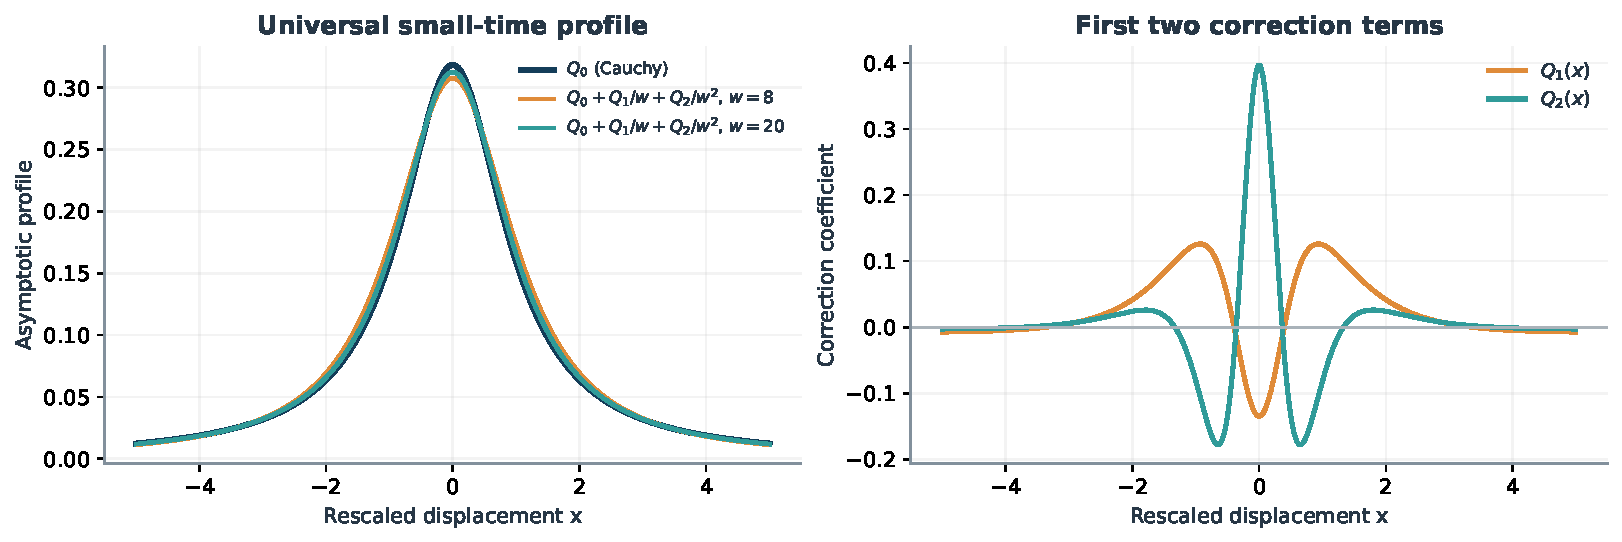
\includegraphics[width=\textwidth]{figures/universal_profiles.pdf}
 \caption{The universal Cauchy profile and its first two corrections.
 The displayed finite expansions are analytic asymptotic profiles, not
 numerical evaluations of the exact transition density at a chosen
 time. The theorem supplies the approximation and its error.}
 \label{fig:profiles}
\end{figure}

\subsection{The second result in concrete form}

Theorem~\ref{thm:invisible-pole} defines every coefficient explicitly by
second differences of
\[
 F(x)=x\log x+\frac12 x^{3/5}\sin^2(\pi x^{1/5}).
\]
The resulting remainder is zero at $1,32,243,1024,\ldots$, the fifth
powers, but has positive excursions of order $x^{-2/5}$ between them.
Its Mellin transform has an exactly calculated pole at $s=3/5$.
Consequently, even an infinite collection of perfectly favorable
samples need not imply the continuous one-sided bound used in a
zero-exclusion argument.

The construction respects positivity and a uniform coefficient bound;
it is not based on arbitrarily large isolated weights. It concerns the
general analytic class. Genuine prime weights possess further arithmetic
structure, so the theorem does not settle which sampling patterns that
additional structure might permit.

\section{What is transferred from the repository and the RH overview}

\subsection{Pinned statements and verification boundary}

We inspected revision
\texttt{72fead102f663d5c7a407964a13dc0cf9d977207} of
\texttt{lsernau/grh-lean}~\cite{Repository}.
The readable project pins Lean v4.35.0 and Mathlib revision
\texttt{56a00585} (full hash in the source manifest).
Its five exports are Mathlib's RH, the corresponding zeta zero-line
statement, half-plane nonvanishing of Dirichlet $L$-functions, and two
Dirichlet zero-line formulations. Selected exact source snapshots, including the standalone statements and axiom-inspection driver, are
included in the archive with hashes.

This task inspected those sources and the external verification record;
it did not rebuild the approximately 300,000-line readable development.
The new theorems below are ordinary mathematical proofs. The included
Lean files are attributed upstream snapshots, not a formalization of
our new theorems.

\subsection{A positive remainder and its transform}

Writing $\Lambda$ for the von Mangoldt function and $\chi_d$ for the
quadratic character associated with an admissible auxiliary prime $d$,
the repository uses nonnegative weights
\[
 b_{d,q}(n)=\Lambda(n)(1-\chi_d(n))\mathbf 1_{n\equiv1\pmod q}
\]
and the remainder
\begin{equation}\label{eq:upstream-remainder}
 R_{d,q}(x)=\sum_{n\leq x}b_{d,q}(n)
       \left(\frac1n-\frac1x\right)
       -\frac{\log x}{\varphi(q)}-c_{d,q}.
\end{equation}
The constant is fixed through a pole-removed logarithmic derivative;
its normalization matters. The exact definitions appear in
\texttt{New/Reduction/Zeros/PrimeError.lean}.

In reciprocal coordinates its positivity yields
\[
 R_{d,q}(1/u)-\frac{\log u}{\varphi(q)}
 =\sum_n b_{d,q}(n)(1/n-u)_+-c_{d,q},
\]
a convex function of $u$. The transform
\[
 \int_0^\infty R_{d,q}(e^v)e^{(1-s)v}\,dv
 =\int_1^\infty R_{d,q}(x)x^{-s}\,dx
\]
has residues measuring the difference between the multiplicities of
untwisted and quadratically twisted zeros. A one-sided estimate and a
Landau argument force those residues to vanish; suitable auxiliary
twists remove cancellation. The implementation is in
\texttt{Lib/Analytic/Landau.lean} and
\texttt{New/Reduction/Zeros/Criterion.lean}.

The arithmetic part obtains the required bound by comparing short
integral forms, a spanning estimate, and a determinant lower bound.
Their main terms cancel, leaving a small prime-sum remainder. The
source audit records the exact interface theorem names. Our second
result examines how much information sampled remainder values can
provide before these arithmetic inputs are used.

\subsection{What the overview contributes}

The RH overview~\cite{WikipediaRH} highlights Li positivity, the
explicit formula, and the de Bruijn--Newman constant. Li's criterion
directs us to the unit-circle values $1-1/\rho$; these become the jump
angles in the first result. The explicit-formula viewpoint motivates
tracking actual Mellin poles in the sampling obstruction. The known
deduction that the de Bruijn--Newman constant is zero follows from RH
and Rodgers--Tao~\cite{RodgersTao}; it is not counted as a new result in
this report.

% Self-contained mathematical fragment; requires amsmath, amssymb, amsthm.
% Suggested bibliography keys: Lagarias2007, BMOR2021, NakamuraSuzuki2023.

\section{A universal process built from zero ordinates}

This section separates two facts. The probabilistic theorem below follows
from the classical zero-counting law alone. RH or Dirichlet GRH identifies
the resulting circle generator with the usual Li coefficients. The repository supplies the established zero-line theorem needed for
that identification.

Let $\mathcal Z$ be a locally finite multiset of real numbers, with
multiplicities, and put
\[
 N(T)=\#\{\gamma\in\mathcal Z:|\gamma|\leq T\}.
\]
Assume that, for constants $d>0$ and $B\in\mathbb R$,
\begin{equation}\label{eq:generic-zero-count}
 N(T)=\frac{d}{\pi}T\log T+\frac{B}{\pi}T+O(\log(T+2))
 \qquad(T\longrightarrow\infty).
\end{equation}
Define
\[
 \theta(\gamma)=
 \begin{cases}2\arctan(1/(2\gamma)),&\gamma\ne0,\\
 \pi,&\gamma=0,
 \end{cases}
 \qquad
 \nu=\frac12\sum_{\gamma\in\mathcal Z}
       (\delta_{\theta(\gamma)}+\delta_{-\theta(\gamma)}).
\]
In particular, $m$ occurrences of $\gamma=0$ contribute mass $m/2$ at
each of $\pi$ and $-\pi$. Write
\begin{equation}\label{eq:jump-symbol}
 \Psi(u)=\int_{\mathbb R}(1-\cos(uy))\,\nu(dy)
       =\sum_{\gamma\in\mathcal Z}(1-\cos(u\theta(\gamma))).
\end{equation}

\begin{lemma}[Existence and elementary properties]\label{lem:jump-exists}
The measure $\nu$ is a symmetric L\'evy measure supported in $[-\pi,\pi]$.
It satisfies
\[
 \nu(\mathbb R)=\infty,\qquad
 \int |y|\,\nu(dy)=\infty,\qquad
 0<V:=\int y^2\,\nu(dy)<\infty.
\]
There is a symmetric L\'evy process $(X_t)_{t\geq0}$ with
\[
 \mathbb E e^{iuX_t}=e^{-t\Psi(u)}.
\]
Its Gaussian component is zero, it has infinitely many jumps and infinite
variation, and $\mathbb E X_t^2=tV$.
\end{lemma}

\begin{proof}
The counting law and partial summation show that
$\sum_{|\gamma|>1}|\gamma|^{-2}<\infty$ whereas
$\sum_{|\gamma|>1}|\gamma|^{-1}=\infty$.
Since $|\theta(\gamma)|\sim |\gamma|^{-1}$, all assertions about the
measure follow. L\'evy--Khintchine gives the process, with zero Gaussian
coefficient and zero symmetric drift. The standard variation criterion
for a pure-jump process gives infinite variation. Differentiating the
characteristic function twice at zero gives the variance identity.
\end{proof}

The construction can also be understood by retaining finitely many
ordinates, allowing independent Poisson jumps of each indicated size,
and taking the symmetric limit. The finite second-moment tail makes this
limit well defined; infinitely many small jumps remain in the limit.

\begin{lemma}[The symbol at large frequency]\label{lem:continuous-symbol}
Put $A=d/2$ and $\kappa=\gamma_{\!E}+B/d$, where $\gamma_{\!E}$ is
Euler's constant. Then
\begin{equation}\label{eq:symbol-asymptotic}
 \Psi(u)=A|u|(\log|u|+\kappa)
          +O(\sqrt{|u|}\log(|u|+2))
 \qquad(|u|\longrightarrow\infty).
\end{equation}
\end{lemma}

\begin{proof}
By evenness take $u\geq2$ and set $T=\sqrt u$. The contribution of
$|\gamma|\leq T$ is $O(T\log(T+2))$. On the remaining ordinates,
\[
 \theta(\gamma)=\gamma^{-1}+O(|\gamma|^{-3}),
\]
so the Lipschitz bound for cosine makes the replacement by
$1-\cos(u/\gamma)$ cost at most
\[
 O\left(u\int_T^\infty v^{-3}\,dN(v)\right)=O(\log u).
\]
Let $M(v)=(d v\log v+Bv)/\pi$ and $R(v)=N(v)-M(v)$.
For $g(v)=1-\cos(u/v)$, integration by parts gives
\[
 \int_T^\infty g(v)\,dR(v)
 =-g(T)R(T)-\int_T^\infty R(v)g'(v)\,dv.
\]
The boundary term at infinity vanishes since $g(v)=O(u^2/v^2)$.
As $|g'(v)|\leq u/v^2$, the displayed expression is
\[
 O\left(\log(T+2)+u\int_T^\infty
              \frac{\log(v+2)}{v^2}\,dv\right)
 =O(\sqrt u\log u).
\]
Extending the main integral from $T$ down to zero costs
$O(T\log(T+2))$. Consequently,
\begin{align*}
 \Psi(u)
 &=\frac1\pi\int_0^\infty
     (1-\cos(u/v))(d\log v+d+B)\,dv+O(\sqrt u\log u)\\
 &=\frac u\pi\left[(d\log u+d+B)I_0-dI_1\right]
        +O(\sqrt u\log u),
\end{align*}
where
\[
 I_0=\int_0^\infty\frac{1-\cos y}{y^2}\,dy=\frac\pi2,
 \qquad
 I_1=\int_0^\infty\frac{(1-\cos y)\log y}{y^2}\,dy
     =\frac\pi2(1-\gamma_{\!E}).
\]
For completeness these evaluations follow by differentiating, at
$\alpha=1$, the absolutely convergent identity
\[
 \int_0^\infty(1-\cos y)y^{-1-\alpha}\,dy
 =\frac{\pi}{2\Gamma(1+\alpha)\sin(\pi\alpha/2)},
 \qquad 0<\alpha<2.
\]
One proof of the identity inserts the Laplace representation of
$y^{-1-\alpha}$ and uses Tonelli's theorem and
$\int_0^\infty e^{-ty}(1-\cos y)\,dy=1/[t(1+t^2)]$.
Substitution gives \eqref{eq:symbol-asymptotic}.
\end{proof}

\section{The all-order density expansion}

Let $W_0$ denote the positive real branch of Lambert's function,
characterized by $W_0(z)e^{W_0(z)}=z$ for $z>0$. Define
\begin{equation}\label{eq:generic-scale}
 w(t)=W_0\left(\frac{e^\kappa}{At}\right),\qquad
 a(t)=Atw(t).
\end{equation}
The exact identities
\begin{equation}\label{eq:scale-identities}
 a=e^{\kappa-w},\qquad \log(1/a)+\kappa=w,
 \qquad t=\frac{a}{Aw}
\end{equation}
are the reason to use Lambert $W$ instead of truncating the scale itself.

For $k\geq0$ set
\begin{equation}\label{eq:universal-profiles}
 Q_k(x)=\frac{(-1)^k}{\pi k!}\operatorname{Re}
 \left.
 \frac{\partial^k}{\partial z^k}
       \bigl[\Gamma(z)(1-ix)^{-z}\bigr]
 \right|_{z=k+1}.
\end{equation}
The logarithm implicit in the complex power is the principal logarithm;
its argument always has positive real part.

\begin{theorem}[Universal expansion at every logarithmic order]
\label{thm:all-orders}
For every $t>0$, $X_t$ has a density $f_t$ which extends to an entire
function of its spatial variable. For every pair of fixed integers
$K,r\geq0$,
\begin{equation}\label{eq:all-order-bound}
 \sup_{x\in\mathbb R}
 \left|
 \frac{d^r}{dx^r}
 \left[a(t)f_t(a(t)x)-\sum_{k=0}^K\frac{Q_k(x)}{w(t)^k}\right]
 \right|
 =O_{K,r}\bigl(w(t)^{-K-1}+\sqrt{a(t)}\bigr)
\end{equation}
as $t\downarrow0$. In particular the error is $O_{K,r}(w^{-K-1})$.
The constants may depend on the multiset and its counting estimate.
\end{theorem}

\begin{proof}
The large-frequency estimate makes
$\exp(-t\Psi(u)+c|u|)$ integrable for every $t>0$ and $c>0$.
Fourier inversion therefore gives an entire density.
Put $a=a(t)$, $w=w(t)$, and for $s>0$ define
\[
 F_w(s)=s+\frac{s\log s}{w}.
\]
The scale identities yield
\[
 tA\frac{s}{a}\left(\log\frac{s}{a}+\kappa\right)=F_w(s).
\]
We first establish, for each fixed $r\geq0$,
\begin{equation}\label{eq:fourier-comparison}
 \int_0^\infty s^r
  \left|e^{-t\Psi(s/a)}-e^{-F_w(s)}\right|\,ds
 =O_r(\sqrt a).
\end{equation}
On $0<s<\sqrt a$, the first exponential is at most one. The negative
part of $F_w$ is at most $e^{-w-1}/w$, so the second exponential is
uniformly bounded as well. This interval contributes $O_r(\sqrt a)$.
On $s\geq\sqrt a$, both exponents are at least $cs$ for some fixed
$c>0$, once $t$ is small enough. Indeed
$F_w(s)/s\geq 1/2+\kappa/(2w)$, and the remainder in
\eqref{eq:symbol-asymptotic} is smaller than a fixed fraction of its
main term on $s/a\geq a^{-1/2}$. The exponential mean-value bound now gives
\[
 \left|e^{-t\Psi(s/a)}-e^{-F_w(s)}\right|
 \leq C t\sqrt{s/a}\log(2+s/a)e^{-cs}.
\]
Since $t=a/(Aw)$ and
$\log(2+s/a)\leq w+C_\kappa+\log(2+s)$, its integral against $s^r$
is $O_r(\sqrt a)$, proving \eqref{eq:fourier-comparison}.

Expand $e^{-s\log s/w}$ through degree $K$. For $s\geq1$, Taylor's
integral remainder for $e^{-z}$, $z\geq0$, is bounded by
$z^{K+1}/(K+1)!$. For $0<s<1$, use $|s\log s|\leq1/e$ and the
same estimate with the harmless factor $e^{1/(ew)}$. Multiplication by
$e^{-s}s^r$ and integration show that
\begin{equation}\label{eq:taylor-comparison}
 \int_0^\infty s^r e^{-s}
 \left|e^{-s\log s/w}
  -\sum_{k=0}^K\frac{(-s\log s)^k}{k!w^k}\right|\,ds
 =O_{K,r}(w^{-K-1}).
\end{equation}
The sum of \eqref{eq:fourier-comparison} and
\eqref{eq:taylor-comparison} is an $L^1$ bound for the Fourier
transforms, with every fixed polynomial weight. Fourier inversion and
differentiation prove the uniform claim. Finally,
\[
 \int_0^\infty s^k(\log s)^k e^{-(1-ix)s}\,ds
 =\left.\partial_z^k
       [\Gamma(z)(1-ix)^{-z}]\right|_{z=k+1},
\]
which identifies the profiles. As $a=e^{\kappa-w}$, $\sqrt a$ is
smaller than every fixed inverse power of $w$.
\end{proof}

The first three terms have the explicit form
\begin{align}
 Q_0(x)&=\frac1{\pi(1+x^2)},\label{eq:profile-zero}\\
 Q_1(x)&=-\frac1\pi\operatorname{Re}
       \frac{1-\gamma_{\!E}-\log(1-ix)}{(1-ix)^2},
       \label{eq:profile-one}\\
 Q_2(x)&=\frac1\pi\operatorname{Re}
       \frac{(\frac32-\gamma_{\!E}-\log(1-ix))^2+\frac{\pi^2}6-\frac54}
            {(1-ix)^3}.
       \label{eq:profile-two}
\end{align}
Thus the leading shape is the standard Cauchy density, and the theorem
provides every successive correction rather than only convergence in law.

\begin{corollary}[Universality beyond every logarithmic order]
If two multisets satisfy \eqref{eq:generic-zero-count} with the same
$d,B$, their scaled densities differ by $O_r(\sqrt a)$ in
$C_b^r(\mathbb R)$. In particular they have the same expansion to every
fixed order in $1/\log(1/t)$.
\end{corollary}

\begin{proof}
Both scaled characteristic functions differ from the same model
$e^{-F_w(|s|)}$ by $O_r(\sqrt a)$ in the weighted $L^1$ norm
\eqref{eq:fourier-comparison}. Apply Fourier inversion directly; this
is stronger than subtracting two fixed-order asymptotic expansions.
\end{proof}

\section{Dirichlet characters and Li coefficients}

For zeta, use the normalization
\[\xi(s)=\tfrac12s(s-1)\pi^{-s/2}\Gamma(s/2)\zeta(s),\qquad
\lambda_n=\frac1{(n-1)!}\left.\frac{d^n}{ds^n}
[s^{n-1}\log\xi(s)]\right|_{s=1}.\]
The equivalent zero-sum formula and its Dirichlet generalization
are used below~\cite{Li1997,BombieriLagarias,Lagarias2007}.

Take $\mathcal Z$ to be the ordinates of all nontrivial zeros of a fixed
primitive Dirichlet $L$-function of conductor $q>1$, counted with
multiplicity and both signs. The classical counting law, in the explicit
form of Bennett--Martin--O'Bryant--Rechnitzer~\cite{BMOR2021}, gives
\[
 N_\chi(T)=\frac T\pi\log\frac{qT}{2\pi e}
              +O_\chi(\log(T+2)).
\]
The zeta function is included by taking $q=1$ and its usual
Riemann--von Mangoldt formula. Thus $d=1$,
$B=\log(q/(2\pi))-1$, and the scale is
\begin{equation}\label{eq:dirichlet-scale}
 w_q(t)=W_0\left(\frac{q e^{\gamma_{\!E}-1}}{\pi t}\right),
 \qquad a_q(t)=\frac t2 w_q(t).
\end{equation}
All preceding density statements are unconditional for these ordinate
processes. All primitive characters of a fixed conductor have the same
expansion to every logarithmic order. Constants are for fixed characters;
no uniformity in $q\to\infty$ is asserted.

Under the relevant RH, each zero $\rho=1/2+i\gamma$ satisfies
$1-1/\rho=e^{i\theta(\gamma)}$ (with $e^{i\pi}=-1$ at a central
zero). Hence the usual zero-sum Li coefficient obeys
\begin{equation}\label{eq:li-identification}
 \operatorname{Re}\lambda_\chi(n)
 =\sum_\rho\operatorname{Re}
       \left[1-\left(1-\frac1\rho\right)^n\right]
 =\Psi_\chi(n).
\end{equation}
The real-part sum is absolutely convergent. For real characters the Li
coefficients themselves are real; for nonreal characters the real part
in \eqref{eq:li-identification} is essential.

The link with Li coefficients and positivity has substantial precedent~\cite{Lagarias2007,NakamuraSuzuki2023}.
The all-order normalized density expansion, rather than the existence
of positive kernels alone, is the proposed contribution here.

\section{The circle kernel and its trace}

Reduce $X_t$ modulo $2\pi$ and let $p_t$ be its density with respect to
ordinary Lebesgue measure on $[-\pi,\pi]$. Its Fourier series is
\begin{equation}\label{eq:circle-kernel}
 p_t(y)=\frac1{2\pi}\sum_{n\in\mathbb Z}e^{-t\Psi(n)}e^{iny}.
\end{equation}
The series converges locally uniformly for complex $y$, so the density
is entire and periodic. Under RH or GRH the associated nonnegative generator has eigenvalues
$\operatorname{Re}\lambda_\chi(|n|)$, with $\lambda_\chi(0)=0$.

\begin{proposition}[Local circle expansion and heat trace]
For every fixed $R>0$ and integers $K,r\geq0$,
\[
 \sup_{|x|\leq R}\left|
 \frac{d^r}{dx^r}
 \left[ap_t(ax)-\sum_{k=0}^K\frac{Q_k(x)}{w^k}\right]
 \right|=O_{R,K,r}(w^{-K-1}+\sqrt a).
\]
If $\mathcal A$ is the circle generator, then
\begin{align*}
 \operatorname{Tr}(e^{-t\mathcal A})
 &=2\pi p_t(0)\\
 &=\frac2a\left[
 1-\frac{1-\gamma_{\!E}}w
 +\frac{(\frac32-\gamma_{\!E})^2+\frac{\pi^2}6-\frac54}{w^2}
 +O(w^{-3})\right].
\end{align*}
For a primitive Dirichlet character the leading trace is
$4/(t w_q(t))$.
\end{proposition}

\begin{proof}
The scaled sum \eqref{eq:circle-kernel} has mesh $a$ in frequency.
Splitting at $an=\sqrt a$ and applying the same mean-value estimates
as in \eqref{eq:fourier-comparison} bounds its difference from the
model Riemann sum by $O_r(\sqrt a)$. The model function
$s^r e^{-F_w(s)}e^{ixs}$ has uniformly integrable first derivative for
$|x|\leq R$; the only possible singularity is an integrable logarithm
at zero. The Riemann-sum error is consequently $O_{R,r}(a)$.
The Taylor calculation is unchanged. Setting $x=0$ gives the trace.
\end{proof}

Uniformity over all real $x$ in the circle assertion would be false:
periodicity produces returning peaks at distances $2\pi/a$. The
whole-line theorem has no such restriction.

\section{A moment transition and two different time scales}

The Cauchy limit does not contradict the finite variance of $X_t$.
The family loses uniform integrability after the short-time
normalization. The following formulas quantify the change.

\begin{theorem}[Moment transition]\label{thm:moment-transition}
Let $L=\log(1/t)$ and retain $A=d/2$. As $t\downarrow0$,
\begin{align*}
 \mathbb E|X_t|^p
 &\sim \frac{a(t)^p}{\cos(\pi p/2)},&&0<p<1,\\
 \mathbb E|X_t|
 &\sim \frac A\pi tL^2
       =\frac d{2\pi}tL^2,&&p=1,\\
 \mathbb E|X_t|^p
 &\sim t\int |y|^p\nu(dy),&&1<p<2,\\
 \mathbb E X_t^2&=tV.&&
\end{align*}
Moreover
\[
 \frac{X_t}{a(t)}\ \Longrightarrow\ \mathrm{Cauchy}(0,1)
 \quad(t\downarrow0),\qquad
 \frac{X_t}{\sqrt{tV}}\ \Longrightarrow\ N(0,1)
 \quad(t\longrightarrow\infty).
\]
\end{theorem}

\begin{proof}
For $0<p<2$ the fractional-moment identity is
\[
 \mathbb E|X_t|^p
 =c_p\int_0^\infty(1-e^{-t\Psi(u)})u^{-p-1}\,du,
 \qquad c_p=\frac{2\Gamma(1+p)\sin(\pi p/2)}\pi.
\]
It follows by Tonelli from the cosine integral evaluated in
Lemma~\ref{lem:continuous-symbol}. For $0<p<1$ put $u=s/a$.
For a sufficiently large fixed $U_0$, the interval $s\leq aU_0$
contributes $O(t a^{-p})=o(1)$ to the normalized moment, using
$\Psi(u)\leq Vu^2/2$. On $aU_0\leq s\leq1$, the symbol bound gives
$t\Psi(s/a)\leq Cs$; on $s\geq1$ use $1-e^{-t\Psi}\leq1$.
Dominated convergence then gives
\[
 \lim_{t\downarrow0}\frac{\mathbb E|X_t|^p}{a^p}
 =c_p\int_0^\infty(1-e^{-s})s^{-p-1}\,ds
 =\frac1{\cos(\pi p/2)}.
\]
For $1<p<2$, divide the unscaled identity by $t$ and use
$(1-e^{-t\Psi})/t\leq\Psi$. The bound
$\Psi(u)=O(u^2)$ at zero and \eqref{eq:symbol-asymptotic} at infinity
provide an integrable majorant. Tonelli identifies the limit with
$\int|y|^p\nu(dy)$.

At $p=1$, the part $0<u<1$ is $O(t)$. For an upper bound split at
$U=1/t$, use $1-e^{-z}\leq\min(z,1)$, and obtain
\[
 \mathbb E|X_t|
 \leq \frac{2t}\pi\int_1^{1/t}\frac{\Psi(u)}{u^2}\,du+O(t)
 =\frac A\pi tL^2+O(tL).
\]
For a lower bound retain only $1\leq u\leq1/(tL^2)$ and use
$1-e^{-z}\geq z-z^2/2$. The main term is
$\frac A\pi t(L-2\log L)^2+O(tL)$; the quadratic error is $O(t)$,
since $t^2\int_1^{1/(tL^2)}\Psi(u)^2u^{-2}\,du=O(t)$.
These two bounds give the claimed equivalent. The variance identity
was proved earlier.

The short-time weak limit follows from
$t\Psi(s/a)\to|s|$. For long times, dominated convergence in the
L\'evy integral gives $\Psi(u)=Vu^2/2+o(u^2)$ as $u\to0$.
Consequently $t\Psi(s/\sqrt{tV})\to s^2/2$, which proves the
Gaussian limit by the continuity theorem.
\end{proof}



\clearpage
% Supplementary result: a bounded-coefficient obstruction to sparse sampling.
% Prepared independently from the repository's one-sided prime-sum mechanism.
% Requires amsmath, amssymb, amsthm; theorem/proof environments provided by parent.

\section{A bounded-coefficient obstruction to sparse sampling}
\label{sec:sampling-obstruction}

The one-sided analytic criterion in \texttt{grh-lean} applies to a
positively weighted, smoothed arithmetic sum.  Positivity also permits
interpolation between sampled values.  The fourth-power sampling principle
itself is already in Setiawan's November 2026 preprint~\cite{Setiawan2026}: its Sections~3 and~4
use convexity to recover a continuous bound from
suitably spaced samples.  The same preprint includes single-interval
sharpness for convex interpolation.  We do not claim those statements as
new.  The theorem below supplies a different strengthening of the
obstruction: one globally defined sequence, bounded positive coefficients,
exactly vanishing samples at \emph{every} fifth power, and a genuine Mellin
pole that all those samples miss.

\begin{theorem}[Bounded positive coefficients with an invisible pole]
\label{thm:invisible-pole}
There is an explicitly defined sequence of real numbers $(a_n)_{n\geq1}$
with
\[
                         0<a_n<4
\]
such that the function
\[
 R(x)=\sum_{n\leq x}a_n\left(\frac1n-\frac1x\right)-\log x,
                    \qquad x\geq1,
\]
has all the following properties.
\begin{enumerate}
\item $R(m^5)=0$ for every positive integer $m$.
\item For every $x\geq1$,
\[
0\leq R(x)-\frac12 x^{-2/5}\sin^2(\pi x^{1/5})
                       \leq \frac1{2x^2}.
\tag{S1}\label{eq:sampling-error}
\]
In particular $R\geq0$, $R(x)=O(x^{-2/5})$, and, for every
$\beta<3/5$, the upper estimate $R(x)=O_+(x^{\beta-1})$ is false.
\item The Mellin transform
\[
                  \Phi(s)=\int_1^\infty R(x)x^{-s}\,dx
\]
is absolutely convergent for $\Re s>3/5$.  It has a meromorphic
continuation to $\Re s>-1$ whose only pole is a simple pole at $s=3/5$,
with residue $1/4$.
\end{enumerate}
The notation $O_+$ means an upper bound with a fixed positive constant;
no lower bound is intended.  The coefficients are real numbers indexed
by integers, not integer-valued coefficients.
\end{theorem}

\begin{proof}
Define, for $x\geq1$,
\[
 h(x)=x^{3/5}\sin^2(\pi x^{1/5}),\qquad
 F(x)=x\log x+\frac12h(x).
\]
Thus $F(1)=0$.  Set
\[
 a_1=F(2),\qquad
 a_n=n\bigl(F(n+1)-2F(n)+F(n-1)\bigr)\quad(n\geq2).
\tag{S2}\label{eq:explicit-coefficients}
\]
These formulas define every coefficient without a limiting choice.

We first verify positivity and the uniform bound.  Differentiation gives
\begin{align*}
 xh''(x)={}&-\frac6{25}x^{-2/5}\sin^2(\pi x^{1/5})\\
 &+\frac{2\pi}{25}x^{-1/5}\sin(2\pi x^{1/5})
   +\frac{2\pi^2}{25}\cos(2\pi x^{1/5}).
\end{align*}
Consequently, using $x\geq1$ and $\pi<4$,
\[
 |xh''(x)|\leq\frac{6+2\pi+2\pi^2}{25}<\frac{46}{25}.
\]
It follows that
\[
              \frac{2}{25x}<F''(x)<\frac{48}{25x}<\frac2x.
\tag{S3}\label{eq:convexity-bounds}
\]
For $n\geq2$, the standard second-difference identity
\[
 F(n+1)-2F(n)+F(n-1)
   =\int_{-1}^{1}(1-|u|)F''(n+u)\,du
\]
now proves
\[
            0<a_n<\frac{2n}{n-1}\leq4.
\]
Also $0<a_1=2\log2+\tfrac12 2^{3/5}\sin^2(\pi2^{1/5})<3$.

Let $IF$ be the continuous function that agrees with $F$ at every
positive integer and is affine between consecutive integers.  Its slope
on $[m,m+1]$ is $F(m+1)-F(m)$.  The function
\[
                  Q(x)=\sum_{n\leq x}a_n(x/n-1)
\]
has the same initial value $Q(1)=0$ and, on that interval, its slope is
\begin{align*}
 \sum_{n\leq m}\frac{a_n}{n}
 &=F(2)+\sum_{n=2}^{m}\bigl(F(n+1)-2F(n)+F(n-1)\bigr)\\
 &=F(m+1)-F(m).
\end{align*}
Thus $Q=IF$ on $[1,\infty)$ and
\[
 R(x)=\frac{IF(x)}x-\log x
     =\frac12x^{-2/5}\sin^2(\pi x^{1/5})+\varepsilon(x),
 \qquad
 \varepsilon(x)=\frac{IF(x)-F(x)}x.
\tag{S4}\label{eq:decomposition}
\]
Since $F$ is convex, $\varepsilon\geq0$.  On $[m,m+1]$,
\eqref{eq:convexity-bounds} and the elementary chord-error bound give
\[
0\leq IF(x)-F(x)
 \leq\frac{(x-m)(m+1-x)}m\leq\frac1{4m}.
\]
Dividing by $x$, and using $x\leq m+1\leq2m$, gives
$0\leq\varepsilon(x)\leq1/(2x^2)$.  At every integer $x$,
$\varepsilon(x)=0$.  In particular, $x=m^5$ makes both terms in
\eqref{eq:decomposition} zero, proving the exact sample identities.

At $x_m=(m+\tfrac12)^5$, however, the sine-squared term equals one, so
\[
             \frac{R(x_m)}{x_m^{\beta-1}}
                    \geq\frac12 x_m^{3/5-\beta}\longrightarrow\infty
                    \qquad(\beta<3/5).
\]
This proves the failure of the proposed continuous upper bound.

It remains to prove the claimed analytic continuation, rather than merely
infer a singularity from the size of the intervening humps.  By
\eqref{eq:sampling-error},
\[
                 H(s)=\int_1^\infty\varepsilon(x)x^{-s}\,dx
\]
is holomorphic in $\Re s>-1$, by absolute convergence uniformly on compact
subsets (the same estimate permits differentiation under the integral).
The identity $\sin^2t=(1-\cos2t)/2$ and the substitution $x=y^5$ give,
initially for $\Re s>3/5$,
\[
 \Phi(s)=\frac1{4(s-3/5)}
          -\frac54 I(2-5s)+H(s),
 \qquad
 I(z)=\int_1^\infty y^z\cos(2\pi y)\,dy.
\tag{S5}\label{eq:pole-decomposition}
\]
Initially $I$ is absolutely convergent for $\Re z<-1$.  Two integrations
by parts give there
\[
               I(z)=-\frac{z}{4\pi^2}
                     -\frac{z(z-1)}{4\pi^2}I(z-2).
\tag{S6}\label{eq:oscillatory-continuation}
\]
The boundary terms at infinity vanish in this half-plane, and at $1$ we
used $\sin(2\pi)=0$ and $\cos(2\pi)=1$.  Repeatedly applying
\eqref{eq:oscillatory-continuation} continues $I$ holomorphically to every
half-plane $\Re z<2N-1$.  There are no variable denominators, so these
continuations are entire and agree on overlaps by the identity theorem.
Hence the last two terms in \eqref{eq:pole-decomposition} are holomorphic
on $\Re s>-1$.  The first term is the asserted unique simple pole and has
residue $1/4$.
\end{proof}

\paragraph{What the obstruction establishes.}
For any $1/2<\beta<3/5$, all the sample bounds
$R(m^5)\leq m^{5(\beta-1)}$ hold, even with a zero left-hand side, while
the Mellin transform has a positive real residue at a pole to the right
of $\beta$.  Thus positivity, uniformly bounded coefficients, exact
fifth-power observations, and meromorphic continuation across the
relevant half-plane do not suffice to reconstruct the one-sided estimate
needed by a Landau argument.  The actual von Mangoldt weights have more
arithmetic structure; this example does not rule out exploiting that
structure in a sparser criterion.  The continuation proved here is to
$\Re s>-1$.  We do not assert that this construction satisfies the exact
whole-plane \texttt{IsPolar} definition in the Lean repository.

\paragraph{A family of examples.}
The same construction works with every integer $p\geq4$, replacing
$3/5$ by $1-2/p$, $x^{1/5}$ by $x^{1/p}$, and fifth powers by $p$th
powers.  The pole lies at $1-2/p$ and still has residue $1/4$.
Indeed, writing $r=1/p$, the analogue of the second-derivative bound is
\[
 |xh_p''(x)|\leq 2r(1-2r)+\pi r(1-3r)+2\pi^2r^2
 =C_p:=\frac{2+\pi}{p}+\frac{2\pi^2-3\pi-4}{p^2}.
\]
Both coefficients in the last expression are positive, so $C_p$ decreases
for $p\geq4$.  Moreover
$C_4=1/4+\pi/16+\pi^2/8<2$, for example using $\pi<22/7$.
Thus $0<F_p''(x)<2/x$ and the same bounds on the weights follow.
The interpolation error remains $O(x^{-2})$, and the oscillatory Mellin
term is $-(p/4)I(p(1-s)-3)$, which is entire in $s$.


\begin{figure}[htbp]
 \centering
 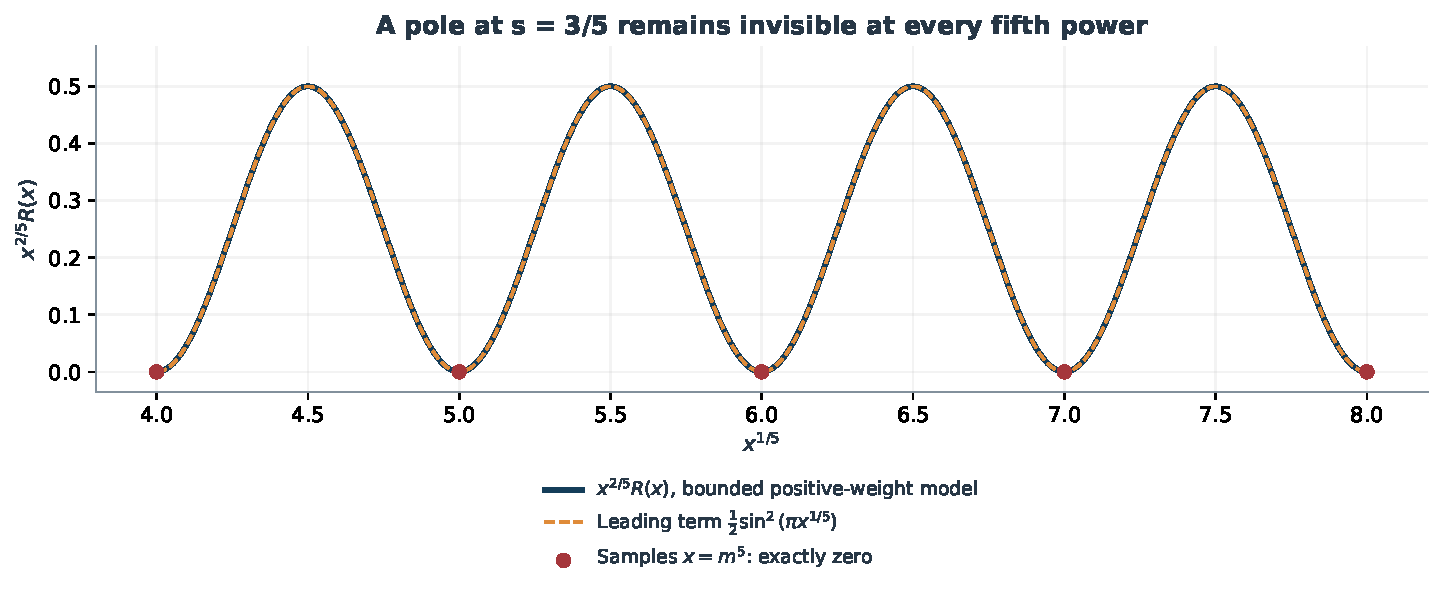
\includegraphics[width=\textwidth]{figures/invisible_pole.pdf}
 \caption{The explicit bounded positive-weight example, plotted in the
 coordinate $x^{1/5}$. Every integer on this horizontal axis is an
 exactly vanishing fifth-power sample. The intervening excursions
 produce the Mellin pole at $3/5$.}
 \label{fig:sampling}
\end{figure}

\section{Novelty and relation to existing work}\label{sec:novelty}

The new claims are deliberately attached to precise statements.
Li's zero-sum criterion and its generalizations are established
work~\cite{Li1997,BombieriLagarias,Lagarias2007}. Lagarias also constructs
an entire interpolation of the Li coefficients, identifies its
frequency support in the angle interval, and proves the familiar
$n\log n$ asymptotics. Passing from a nonnegative cosine sum to a
symmetric convolution semigroup is a standard use of
L\'evy--Khintchine theory. These ingredients are not claimed as new.

Nakamura--Suzuki already relate RH to infinitely divisible
distributions~\cite{NakamuraSuzuki2023}. Their construction uses zero
ordinates with inverse-square weights. Here the measure has equal
symmetrized weights at transformed angles, infinitely many small jumps,
and the quantitative question is an explicit all-order density and
trace expansion. The relation between Li coefficients and Hilbert-space
norms is also established~\cite{Suzuki2023}.

General small-time moment limits for L\'evy processes have a substantial
literature~\cite{FigueroaLopez2008}. The moment transition here is an
explicit specialization with a self-contained proof and a computed
critical coefficient. The central contribution is
Theorem~\ref{thm:all-orders}: the Lambert-$W$ normalization, all of the
profiles $Q_k$, the uniform differentiated remainder, and the resulting
conductor universality and trace formulas as one precise theorem.

For sampling, Setiawan's v2 preprint already proves fourth-power
sufficiency at the square-root scale and local convex interpolation
sharpness~\cite{Setiawan2026}. Exact logarithmic chord maxima can also
be expressed through the classical Specht ratio~\cite{Seo2010}. We therefore do not
claim the basic interpolation exponent or its local sharpness.
The proposed contribution is the global construction in
Theorem~\ref{thm:invisible-pole}: bounded positive coefficients, exact
zeros on the complete prescribed grid, and a uniquely identified
Mellin pole with explicit residue.

Targeted searches covered Li semigroups, Cayley-angle distributions,
heat kernels and heat traces, small-time Cauchy limits, Lambert-$W$
scalings, and sparse RH sampling. No source located in this
investigation states the two precise theorems proved here. This is a
documented novelty assessment, not a certification of worldwide
priority. A related SSRN abstract on reciprocal $\xi$ and $\zeta$
distributions was located, but its full text was inaccessible; it has
not been treated as fully audited. The novelty of semigroup existence
is not relied on in any case.

\section{Reproduction, checks, and formalization map}

The complete arguments use classical zero counting, calculus,
Stieltjes integration by parts, Fourier inversion, and standard
probability existence results. No numerical hypothesis enters either
main proof. Zeros need not be simple, and the Dirichlet formulation
allows complex characters and central zeros.

The archive contains the editable LaTeX source and all included
sections, the compiled PDF, mathematical figures in PDF and PNG,
Python programs, JSON and CSV outputs, and the pinned source audit.
Run the following from the extracted archive directory:
\begin{verbatim}
python3 code/verify_results.py
python3 code/make_figures.py
python3 code/verify_sampling_obstruction.py --output data
latexmk -pdf -interaction=nonstopmode rh_li_universality.tex
\end{verbatim}
The Python checks use NumPy, SciPy, SymPy, mpmath, and Matplotlib.
The first program verifies the symbolic derivative identity, compares
15 profile integrals with their Gamma-derivative formulas, checks nine
Lambert-scale identities, and examines 30,000 coefficients. The
independent high-precision sampling program checks 3,000 coefficients
and the interpolation formulas at 80-digit precision. These finite
checks support reproducibility; the global positivity and pole
statements follow from the proofs.

The plotted Fourier comparison, where used in the numerical outputs,
is the analytic comparison integral in the proof. It is not asserted
to be an exact transition density. The main figures show the universal
profiles and the explicitly defined sampling example.

A future Lean formalization has two natural independent units. The
sampling theorem can start from finite-difference identities,
convexity, and parameter-dependent integrals. The density theorem
needs a general symmetric-jump construction, an abstract counting-law
lemma, weighted Fourier $L^1$ estimates, and an asymptotic scale
interface. The imported RH/Dirichlet-GRH theorem is used only when
identifying the integer exponents with Li coefficients. This map
identifies the remaining formal work; no unproved Lean stub is
presented as verification.

\begingroup
\small
\begin{thebibliography}{99}
\bibitem{Repository}
L. Sernau and collaborators,
\emph{GRH for Dirichlet L-functions, in Lean 4},
repository \texttt{lsernau/grh-lean}, revision
\texttt{72fead102f663d5c7a407964a13dc0cf9d977207} (25 November 2026).
\url{https://github.com/lsernau/grh-lean}.

\bibitem{LeanStatement}
Lean FRO and Mathlib Initiative,
\emph{Lean verification of the Riemann Hypothesis},
joint statement, 21 November 2026.
\url{https://leanprover-community.github.io/blog/posts/riemann-hypothesis/}.

\bibitem{Rubinstein}
M. Rubinstein, \emph{Alp\"oge/Claude proof of the Generalized Riemann
Hypothesis}, verification account, accessed 26 November 2026.
\url{https://www.math.uwaterloo.ca/~mrubinst/alpoge_claude_grh/}.

\bibitem{WikipediaRH}
Wikipedia contributors, \emph{Riemann hypothesis}, accessed
26 November 2026. Starting overview; technical inputs checked against
primary sources. \url{https://en.wikipedia.org/wiki/Riemann_hypothesis}.

\bibitem{Li1997}
X.-J. Li, The positivity of a sequence of numbers and the Riemann
hypothesis, \emph{J. Number Theory} \textbf{65} (1997), 325--333.
\url{https://doi.org/10.1006/jnth.1997.2137}.

\bibitem{BombieriLagarias}
E. Bombieri and J. C. Lagarias, Complements to Li's criterion for the
Riemann hypothesis, \emph{J. Number Theory} \textbf{77} (1999), 274--287.
\url{https://doi.org/10.1006/jnth.1999.2392}.

\bibitem{Lagarias2007}
J. C. Lagarias, Li coefficients for automorphic $L$-functions,
\emph{Ann. Inst. Fourier} \textbf{57} (2007), 1689--1740.
\url{https://doi.org/10.5802/aif.2311}.

\bibitem{BMOR2021}
M. A. Bennett, G. Martin, K. O'Bryant, and A. Rechnitzer,
Counting zeros of Dirichlet $L$-functions,
\emph{Math. Comp.} \textbf{90} (2021), 1455--1482.
\url{https://arxiv.org/abs/2005.02989}.

\bibitem{NakamuraSuzuki2023}
T. Nakamura and M. Suzuki, On infinitely divisible distributions
related to the Riemann hypothesis,
\emph{Statist. Probab. Lett.} \textbf{201} (2023), 109889.
\url{https://arxiv.org/abs/2306.08317}.

\bibitem{Suzuki2023}
M. Suzuki, Li coefficients as norms of functions in a model space,
\emph{J. Number Theory} \textbf{252} (2023), 177--194.
\url{https://arxiv.org/abs/2301.05779}.

\bibitem{FigueroaLopez2008}
J. E. Figueroa-L\'opez, Small-time moment asymptotics for L\'evy
processes, \emph{Statist. Probab. Lett.} \textbf{78} (2008), 3355--3365.
\url{https://doi.org/10.1016/j.spl.2008.07.012}.

\bibitem{Setiawan2026}
S. Setiawan, \emph{The Primacohedron Trace Formulation of the Riemann
Hypothesis: A Guide to Reconstructing the Alp\"oge--Claude Proof in Lean},
preprint, version 2, posted 25 November 2026.
\url{https://doi.org/10.20944/preprints202611.0738.v2}.

\bibitem{Seo2010}
Y. Seo, A generalized P\'olya--Szeg\H{o} inequality for the Hadamard
product, \emph{Scientiae Mathematicae Japonicae} \textbf{72} (2010),
165--169. See the Specht-ratio formula.
\url{https://www.jstage.jst.go.jp/article/isms/72/2/72_165/_pdf/-char/ja}.

\bibitem{RodgersTao}
B. Rodgers and T. Tao, The de Bruijn--Newman constant is non-negative,
\emph{Forum Math. Pi} \textbf{8} (2020), e6.
\url{https://arxiv.org/abs/1801.05914}.
\end{thebibliography}
\endgroup
\end{document}
